% !TeX spellcheck = de_DE_frami
\documentclass{uebungsblatt}

\providecommand{\dozent}{Fabian Ostermann}
\providecommand{\titel}{Übungsblatt zu\\
	-- Automatische Komposition --}
\providecommand{\untertitel}{Vorlesung Musikdatenanalyse\\WiSe\,22/23}
\providecommand{\ausgabedatum}{27.01.2023}

\usepackage{todonotes}
\newcommand{\todobox}[2][]{\todo[inline, #1]{#2}}

\loesungverbergen
\begin{document}

\begin{center}
	\fbox{
	\begin{minipage}{.75\textwidth}
		\underline{\textbf{Hinweise zur Bearbeitung}}: Das Lösen der folgenden Aufgaben ist generell auf symbolischer Ebene in jeder Programmiersprache (z.B. R oder Matlab) möglich. D.h. die Konsolenausgabe einer symbolischen String-Repräsentation der Musik wie z.B. \texttt{'g4 e4 e2'} (sprich \enquote{g als Viertelnote...}) oder als MIDI-Tonhöhen \texttt{67 64 64} für \raisebox{-.4\baselineskip}{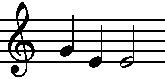
\includegraphics[height=1.5\baselineskip]{img/HaenschenKlein_firstbar.pdf}} ist als Lösung möglich. Eine Hörbarmachung ist dann durch manuelles Spielen auf einem Instrument oder durch manuelle Übertragung in ein Notensatzprogramm (wie z.B. \emph{MuseScore}) möglich.
		\medskip
		
		Ich empfehle jedoch die Bearbeitung der Aufgaben in der Programmiersprache \texttt{Python} mithilfe des Moduls \texttt{scamp}. Die übersichtliche Installation (bei Bedarf inkl. Programmierumgebung \emph{Thonny}) ist gut dokumentiert (siehe \url{http://scamp.marcevanstein.com/narrative/easy_setup.html}) und die Vertonung und sogar Vernotung der generierten Musik geht mit diesem Tool leicht von der Hand. Ein weitreichendes Einstiegstutorial findet sich hier: \url{http://scamp.marcevanstein.com/}.
	\end{minipage}
	}
\end{center}

\begin{loesung}
	Lösungen zu den Code-Aufgaben finden sich in den Ordnern \texttt{code-loesung/aufgabe1/}, \texttt{code-loesung/aufgabe2/} und \texttt{code-loesung/aufgabe3/}.
\end{loesung}

\begin{aufgabe}{Lindenmayer-System}
	
	In dieser Aufgabe soll das Lindenmayer-System aus der Vorlesung (Folien 17--18) implementiert werden.
	
	\begin{teilaufgabe}
		Implementieren Sie das L-System $G = (V$$=$$\{a,b\}, S$$=$$\emptyset, \omega$$=$$a, P$$=$$\{a\mapsto b,b\mapsto ab\})$.\\
		Als Eingabe soll die Anzahl an Interationen $n$ übergeben werden.
	\end{teilaufgabe}
	\begin{tipp}
		Arbeiten Sie mit Strings. {\emph{Achtung}}: String-Funktionen wie \texttt{replace} oder \texttt{replaceAll} sind hier meist nicht hilfreich!
	\end{tipp}
	
	\begin{teilaufgabe}
		Implementieren Sie eine Übersetzung der Variablen $a$ und $b$ auf die Noten $A'$ und $B'$ bzw. deren MIDI-Tonhöhen \texttt{57} und \texttt{59}.
	\end{teilaufgabe}

	\begin{teilaufgabe}
		Überlegen Sie sich und implementieren Sie die Übersetzung der Variablen auf einfache Phrasen (vgl. Vorlesungsfolie 18).
	\end{teilaufgabe}

	\begin{teilaufgabe}
		\emph{Experimentieren Sie}: Ändern Sie das Startwort, die Anzahl an Iterationsschritten $n$ oder auch Variablenanzahl und Produktionsregeln.
	\end{teilaufgabe}
	
\end{aufgabe}

\pagebreak

\begin{aufgabe}{Markov-Ketten}
	In dieser Aufgabe sollen die Markov-Modelle aus der Vorlesung (Folien 20--22) implementiert werden.\\
	Das Stück \enquote{Hänschen Klein} ist als Liste \texttt{hk} von MIDI-Tonhöhen gegeben (Noten finden sich auf~Vorlesungsfolie 21):
	\medskip
	
	\verb|hk = [ 67, 64, 64, 65, 62, 62, 60, 62, 64, 65, 67, 67, 67,|\\
	\verb|       67, 64, 64, 65, 62, 62, 60, 64, 67, 67, 60,|\\
	\verb|       62, 62, 62, 62, 62, 64, 65, 64, 64, 64, 64, 64, 65, 67,|\\
	\verb|       67, 64, 64, 65, 62, 62, 60, 64, 67, 67, 60 ]|
	\begin{teilaufgabe}
		Implementieren Sie ein Programm, dass die Noten zufällig aus der Liste zieht.
	\end{teilaufgabe}
	\begin{tipp}
		Nutzen Sie in Python die Funktion \texttt{random.choice(list)}. Importieren Sie vorher das Modul (\texttt{import random}).
	\end{tipp}

	\begin{teilaufgabe}
		Generieren Sie nun eine Wahrscheinlichkeitsverteilung aus der Liste \texttt{hk}, bei der der Folgezustand (\enquote{zu erzeugende Note}) vom aktuellen Zustand (\enquote{davor erzeugte Note}) abhängt (vgl. Vorlesungsfolie 22).
	\end{teilaufgabe}

	\begin{teilaufgabe}
		Welche möglichen \emph{Tonparameter} werden von diesem konkreten Modell \underline{nicht} berücksichtigt?
		\begin{tipp}
			Ein Beispiel sind \enquote{fehlende} Dynamikvorgaben (Lautstärke) wie \textit{mf} oder \textit{p}.
		\end{tipp}
		\begin{loesung}
			Weitere Attribute sind z.B.: Notenwerte (Länge/Dauer), Tempo, Bendings (ungerade Tonhöhen), Dynamik (Lautstärke), Artikulation, Instrumentierung, Timbre, Mehrstimmigkeit, ...
		\end{loesung}
	\end{teilaufgabe}
	
\end{aufgabe}

\begin{aufgabe}{Expertensystem}
	\begin{teilaufgabe}
		\underline{Parallel Harmony:} Erzeuge für jede Note der Melodie aus Aufgabe~2 einen 4-stimmigen Akkord, der sich ungeachtet des harmonischen Kontexts in reinen Quarten unter die Note schichtet (ein sogenannter Quartakkord).
		\begin{tipp}
			Ein Beispiel: Für die Note $e$ (MIDI-Tonhöhe \texttt{64}) ist es der Akkord $\{c^\sharp,f^\sharp,b,\textbf{e}\}$\footnote{$b$ ist in englischer Schreibweise angegeben und entspricht dem deutsch $h$} (MIDI-Tonhöhen \texttt{[49,54,59,64]}).
		\end{tipp}
	\end{teilaufgabe}
	\begin{teilaufgabe}
		\underline{Tonika und Dominante}: Unterlege die Noten $c$, $e$ und $g$ mit einem C-Dur-Akkord (Tonika, MIDI-Noten \texttt{[48,52,55]}) und die Noten $d$ und $f$ mit einem G-Dur-Akkord (Dominante, MIDI-Noten \texttt{[43,47,50,53]}).
	\end{teilaufgabe}
	\begin{teilaufgabe}
		\underline{Tonika und Dominante pro Takt}: Eine typische Harmonisierung des Stücks nutzt ausschließlich den Tonika-Akkord C-Dur und die Dominante G-Dur. Überlege und definiere eine heuristische Regel, die bei Eingabe einer Menge von Noten (z.B. Takt 1 $\{g,d,d\}$ oder Takt 3 $\{c,d,e,f\}$) eine sinnvolle Vorhersage eines passenden Akkord macht. Bestimme mit dieser Regel einen passenden Akkord für jeden Takt.
	\end{teilaufgabe}
	\begin{loesung}
		\underline{Mögliche Heuristik}: \emph{Der C-Dur-Akkord ist Tonika der Tonart C-Dur und passt gut zu den Akkord-eigenen Melodietönen. Alle anderen Töne sind Spannungstöne. Zu ihnen passt gut die Dominante (G-Dur), die zurück zur Tonika \enquote{leitet}.}
		
		\medskip
		\underline{Umsetzung}:
		Eine Funktion $f$ weist den Tönen $t$ des C-Dur-Akkords $\{c,e,g\}$ das Gewicht $1$, allen anderen Noten das Gewicht $-1$ zu:
		\[
			f(t) = 
			\begin{cases}
				~1, & \text{wenn } t \in \{c,e,g\}\\
				~-1, & \text{sonst} 
			\end{cases}
		\]
		Eine weitere Funktion $F$ weist einer Menge von Tönen $T$ die Summe der einzelnen Gewichtungen zu.
		\[
			F(T) = \sum_{i=1}^n f(t_i) \qquad \text{mit } t_1, ..., t_n \in T
		\]
		Die Funktion $A$ zur Akkordbestimmung wird dann definiert als:
		\[
			A(T) = 
			\begin{cases}
				~\text{C-Dur-Akkord}, & \text{wenn } A(T) \geq 0\\
				~\text{G-Dur-Akkord}, & \text{sonst} 
			\end{cases}
		\]
		
		Ein Beispiel: $A(\{c,d,e\}) = f(c) + f(d) + f(e) = 1+(-1)+1 = 1$
		
		\medskip
		Implementierung: siehe \texttt{loesung/aufgabe3/expertsystem-c.py}
	\end{loesung}
	\begin{teilaufgabe}
		Mit welchen Verfahren und unter welchen Umständen wäre die Ableitung einer Funktion zur Vorhersage automatisierbar?
	\end{teilaufgabe}
	\begin{loesung}
		Mit einem datenbasierten Lernverfahren und einem Datensatz, der der die gewünschten Harmonisierung als \enquote{Ground Truth} zur Vorhersage beinhaltet (vgl. \emph{Supervised Learning}).
	\end{loesung}
\end{aufgabe}

\begin{aufgabe}{Eigene algorithmische Komposition}
	\emph{Werden Sie kreativ!}
	Implementieren Sie ein (heuristisches) Programm, dass eine originale Komposition entwirft.
	Lassen Sie dabei Ihrer Experimentierfreude freien Lauf und/oder nutzen Sie eine der vorgestellten Ansätze/Methodiken aus der Vorlesung.
	\begin{tipp}
		Starten Sie einfach, z.B. mit dem Entwerfen regelbasierter Heuristiken oder dem Würfeln von Noten aus einer Menge/Liste an Möglichkeiten (z.B. C-Dur-Pentatonik $\{C,D,E,G,A\}$; bzw. als MIDI-Tonhöhen \texttt{cdur=[60,62,64,65,67]}).
	\end{tipp}
	\begin{tipp}
		Kapseln Sie Teile Ihrer Komposition und/oder Generierungsregeln in Funktionen, um diese an beliebigen Stellen im Programmcode wiederverwenden zu können.
	\end{tipp}
	\begin{loesung}
		Beispiele: \href{http://scamp.marcevanstein.com/narrative/music.html}{\texttt{scamp.marcevanstein.com/narrative/music.html}}
		
		Bonus: \enquote{Can ChatGPT write a good melody?} (\href{https://www.youtube.com/watch?v=ogfYRBgzZPU}{\texttt{youtube.com/watch?v=ogfYRBgzZPU}})
	\end{loesung}
\end{aufgabe}
	
\end{document}
